\chapter{Datastream Extraction Tool Manual} \label{appendix-dset-manual}
\captionsetup{margin=10pt,font=large,labelfont=bf,textfont={bf}}

The full version of the Datastream Extraction Tool Manual can be found in the project folder of the Google Drive repository under \url{https://bit.ly/3rB3lqg}. 

\section{Introduction}
The Datastream Extraction Tool is an application that allows the user to download financial data from Thomson Reuters Datastream without the overhead of doing it manually in Excel. The tool was created specifically for large static and time-series requests, and supports long-duration downloads of data. 

\section{Installation}
Please, be aware of the following: 
\begin{itemize}
	\item The application can only be run on Windows computers. It cannot be ported to MacOS or Linux, as the Thomson Reuters Excel add-in is only available for Windows, and also because the VBA (Visual Basic for Applications) version on Unix-based computers is a different one than on Windows computers. 
	\item While the application can generally be run on remote computers as well, it can be rather inconvenient. On the one hand, remote computers tend to be less stable in terms of internet connection and add-in connectivity. And additionally, the remote computers of TUM-SOM have rather poor performance (especially disk access!), which would constrain the data download. Furthermore, remote computers automatically shut down after some time, which makes downloading large data loads problematic. For smaller requests though, that take up to 1 hour of download time, the remote execution should suffice. 
\end{itemize}

\subsection{Prerequisites}
Please make sure that the following environment is established before you proceed with the installation.
\begin{itemize}
	\item Make sure you have a valid \textbf{Microsoft Office Installation}. The application was tested with Office 365, but it should also run with other recent Office environments.
	\item Make sure that \textbf{Thomson Reuters Eikon \& Datastream} is installed. If you install it for the first time, please ensure that the Datastream add-on in the Excel plug-in is enabled. 
	\item Make sure that you have an up-to-date version of \textbf{Python 3} installed. Python 3 is different from Python 2; with Python 2 the application will not work. 
	\item Make sure that in Windows Power Options you select that your PC "never" goes to sleep. Since otherwise this can interrupt long-running downloads. 
\end{itemize}

\subsection{Download}
Follow these steps to install the application on your computer: 
\begin{enumerate}
	\item Download the \textit{Shippable} folder from \url{https://bit.ly/2VfT058} to your computer. Choose a location with enough free space, as the downloaded data will be stored in-place. 
	\item Unzip the downloaded file. You can rename the root folder from \textit{Shippable} to a different name at your convenience. Please, do \textbf{not} rename any of the folders or files inside. Such changes would need to be propagated to the program code. 
	\item In the \textit{Shippable }folder, you will find a file called \textbf{\textit{prerequisites.py}}. You need to run this file with Python. You can do so by e.g. right-clicking on the file, selecting "Open with" and then choosing Python. It will then automatically install external Python packages needed for the app. 
\end{enumerate}

\subsection{Settings}
Finally, you will need to adjust some settings in Excel the first time you install the application. For this purpose, open the file called \textit{RequestTable.xlsm} in the \textit{Shippabl}e folder. 

The first time you open it, you might get prompted to activate file contents or to allow modifications, etc. Please agree to all such messages. 

Further, take care of the following settings: 
\begin{itemize}
	\item Make sure that both the \textit{Thomson Reuters} tab and the \textit{Thomson Reuters Datastream} tab show in the tab panel of the Excel document. 
	\item In the Thomson Reuters tab go to Settings $=>$ Sign-In $=>$ choose to automatically sign-in whenever Office is started. 
	\item Go to File $ => $ Options $ => $ Trust Center $ => $ Trust Center Settings and do: 
	\begin{itemize}
		\item Macro Settings $ => $ select "\textit{Enable all macros}" and check "\textit{Trust access to the VBA project object model}". 
		\item Protected View $ => $ uncheck all boxes except for "\textit{Outlook attachments}". 
		\item Add-ins $ => $ uncheck all boxes.
		\item External Content $ => $ select "\textit{Enable all Data Connections}", "\textit{Enable automatic update for all Workbook Links}", "\textit{Enable all Linked Data Types}".
	\end{itemize}
	\item Go to File $ => $ Options $ =>  $Customize Ribbon $ => $ select \textit{Main Tabs} on the right $ => $ check the \textit{Developer, Add-ins, Thomson Reuters}, and \textit{Thomson Reuters Datastream} tabs. 
	\item Go to File $ => $ Options $ => $ Advanced $ => $ section \textit{General} $ => $ uncheck option \textit{Ask to update automatic links}. 
	\item Go to File $ => $ Options $ => $ Add-ins and make sure that the add-in \textit{Thomson Reuters Eikon - Microsoft Office }is listed among \textit{Active Application Add-ins}. It should be. If not, refer to the Troubleshooting section. 
	\item Press "Alt + F11" (the VBA editor will appear) $ => $ go to Tools $ => $ References $ => $ check the box near "\textit{Microsoft Scripting Runtime}"
\end{itemize}

Now, you should be well set to run the application.

\section{Usage}
You can start the Datastream Extraction Tool by running the file \textbf{\textit{ds\_extraction\_tool.py}} with Python. 

If you encounter a problem, some other prerequisites on your computer might be missing that might not have been covered in this guide. In that case, please contact the project developer. 

\subsection{User Interface}
Once you start the application, the user interface (in the following gui) as in Fig. \ref{fig:gui-2} will show. It has the sections: 
\begin{itemize}
	\item Request Type
	\item Time Frames
	\item Request Datatypes
	\item Data IDs
	\item Request Format
	\item Save Results To
\end{itemize}

\begin{figure}[h]
	\centering
	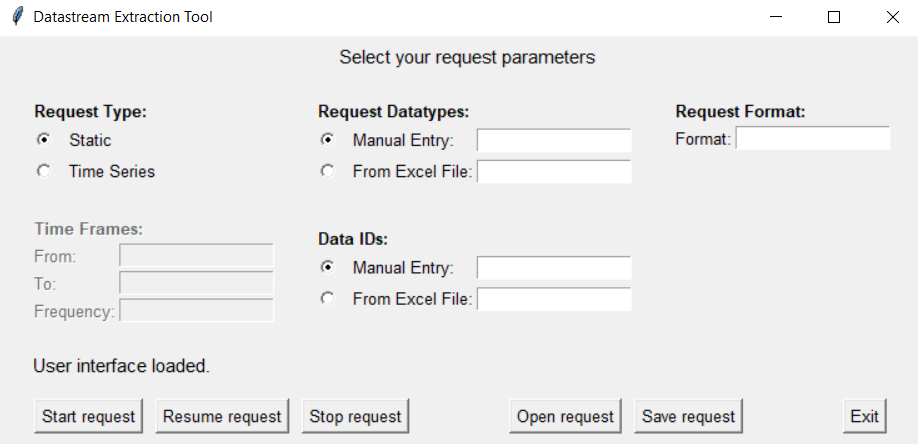
\includegraphics[width=1.1\linewidth]{figures/gui.png}
	\caption{Graphical User Interface of the Datastream Extraction Tool}
	\label{fig:gui-2}
\end{figure}

In the \textbf{Request Type} section you can select your request to encompass either static or time-series data for the stocks or bonds that you want to download. \\

If you select the option \textit{Time Series}, the \textbf{Time Frames} section will become enabled. There, you can enter the start and the end date of the period for which you want to download data. The dates have to be entered in the format "dd/mm/yy" (e.g. 01/01/99 for the 1st of January 1999, or 30/06/20 for the 30th of June 2020). The program assigns year numbers from 51 to 99 automatically to the years 1951 - 1999, and year numbers from 00 to 50 to the years 2000 - 2050. 
In the \textit{Frequency} text field, you can type in the frequency of the time points that you want to get. Here, the values "Daily", "Weekly", "Monthly", "Quarterly", and "Yearly" are allowed. \\

Within the \textbf{Request Datatypes} section, you can enter the codes of the parameter types that you want to get for your stocks or bonds. These could be e.g. "C" for coupon, or "ISIN". You can enter the values either manually, or by choosing the excel file from which you want to get the datatypes. If you choose to enter the datatype codes manually, please do so in a comma-separated manner (e.g. "C,ISIN,AIS,BSTAT"). If you choose to enter the codes via excel file, you have to create an excel file with all the datatype codes listed in column A, one below the other (see Fig. \ref{fig:file-datatypes}). Then, within the app, browse for the created file and select it.

\begin{figure}[h]
	\centering
	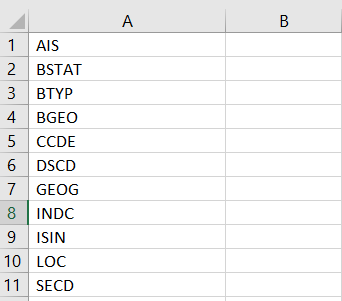
\includegraphics[width=1.1\linewidth]{figures/enter-datatypes.png}
	\caption{A sample file with datatypes}
	\label{fig:file-datatypes}
\end{figure}

In the \textbf{Data IDs} section, you have to enter the datastream codes of the financial instruments - i.e. stocks or bonds - that you are interested in. Just like for datatypes, this can be done either manually, or by giving the excel file name, in which you have previously stored the IDs. When entering them manually, separate the IDs by commas again. When entering them via file, store them in the A column of your excel document, like before, and select the created file in the app by clicking on the "Browse" button. \\

In the \textbf{Request Format} section you can (optionally) enter the format in which you want your data to appear. You can give the format by concatenating the letters of the different format options available in Datastream. For example, "CRM\$" would mean to include column headers (C), row headers (R), instrument code (M), and currency (\$). \\

Finally, in the \textbf{Save Results To} section of the interface you can enter the folder location to which you want your request results to be saved. For this, either enter a valid folder path by hand, or select it by clicking on the button to browse for a suiting folder. \\

Below the parameter sections, there is a \textbf{status bar} that shows you the current status of your request. This can be especially useful for longer requests. Please keep in mind that the status bar can have a delay of up to 2 minutes, depending on the current request phase. For real-time request updates, please refer to Logs in the Folder Structure section of this guide. \\

Additionally, at the bottom of the gui, there are several control buttons. The "\textbf{Start Request}" button first checks the format of the fields you entered, and subsequently launches the request. The current status of the request will be shown in the status bar. \\


The "\textbf{Stop Request}" button shuts down the request if there is one currently running. In its essence, it kills the running Excel instance to stop the data download. Depending on the phase of the request, it might take up to 2 minutes until the request has been stopped. Please abstain from using the gui during this time. \\


The "\textbf{Resume Request}" button is there to resume a request that was previously started and then stopped. This action ignores any entered parameter fields, as it simply resumes the last request, with the settings it has internally saved. Requests that were resumed automatically continue to download data, starting from the last data chunk that has previously been downloaded. Use the "Resume Request" button if your download crushed or if you stopped it manually. \\


The "\textbf{Open Request}" and "\textbf{Save Request}" buttons are there to either save current parameters into a file, or to conveniently load request parameters from a file. Use this for recurring requests to avoid entering them by hand each time. \\


Finally, the "\textbf{Exit}" button first stops the request if there is one running, and then closes the application. If you want to close the application without stopping the request, close the window as usually with the cross at the top right of the window. Note that in this case Excel might proceed running in the background!

\subsection{Application Folders}
The application is shipped with several folders that it requires to run. These are: 

\begin{itemize}
	\item Data
	\item DataTypes
	\item IDs
	\item Logs
	\item PythonPackages
	\item Requests
	\item Settings
\end{itemize}

In \textbf{Data}, the downloaded data from the users' requests is getting stored. It is stored in the form of Excel files. The number of files varies depending on the request size. The file size is centered around 40 MB each, but can also vary, depending on the particular request and the available data. You can use the files with downloaded data for whichever purpose you want. It is advisable though to avoid further manipulating these files in-place, and rather to copy them elsewhere for further processing. \\

In the \textbf{DataTypes} folder, you can put Excel files with the datatypes of financial instruments that you want to download. These have to be stored in column A, one datatype per row. The application is shipped with several examples. \\

In \textbf{IDs}, you can put Excel files containing Datastream identifiers of financial instruments, for which you would like to download data. Just like for datatypes, you have to store these in the A column of the respective Excel file, one ID per row. Refer to section IDs Preparation for hints on how to do it conveniently. \\

In the folder \textbf{Logs}, you will find two files, which are generated when the program is running. The first one is called \textit{log\_python.txt}. It contains real-time information on the progress of the data download. Use the file to either check the current download status, or to track occurring errors, should the application misbehave. The second file is called \textit{log\_request\_table.txt}. It contains real-time information on the progress of the data download on the Excel side of the program (i.e in the request table). You can similarly use it either for progress updates, or for troubleshooting. \\

The folder \textbf{PythonPackages} is of technical nature. It contains python packages that are needed for the application to run. Please, do not touch this folder, unless you know what you are doing. \\

In the folder \textbf{Requests}, you can store parameters of previous requests, in order to reuse these later. The requests are stored .txt files. The file names you can choose yourself at creation. \\

The folder \textbf{Setting}s contains one single file called \textit{settings.txt}. This file is used for multiple purposes, including: 

\begin{itemize}
	\item communication between the python and the excel part of the application
	\item download progress monitoring
	\item error monitoring
	\item status updates in the gui
	\item the "resume request" functionality
\end{itemize}
The settings and communication data within the file is stored in the key-value-format. In most cases, you should \textbf{not} open or modify the file. For exceptions, refer to the Troubleshooting section. 

\subsection{Troubleshooting}

\subsubsection{3.3.1 Thomson Reuters Eikon add-in does not show in the list of active Excel add-ins}
\textbf{Problem Description: }  \\
Thomson Reuters Eikon add-in does not show in the list of active Excel add-ins. \\ \\
\textbf{Solution Proposal:} \\
In the \textit{RequestTable.xlsm} document, navigate to File $ => $ Options $ => $ Add-ins. If the add-in is listed under "Deactivated Application Add-ins" in the Add-ins tab of Options, then at the bottom select \textit{Manage: Deactivated elements} and click on "Go". In the appearing window, if the Thomson Reuters add-in is listed, check it and click on "Activate". \\
If the Reuters add-in is listed under "Inactive Application Add-ins" instead, then at the bottom select \textit{Manage: COM Add-ins} and click "Go". In the appearing window, if \textit{Thomson Reuters Eikon - Microsoft Office} is not checked, check it. If the Reuters add-in is not in the list, click on "Add" and navigate to the add-in location. In many cases, it is stored under 
\url{C:\\Users\\[current_user]\\AppData\\Local\\ThomsonReuters\\Eikon\\EikonOfficeShim.dll}. 
Select it and add it to the list. If not, find out where the file \textit{EikonOfficeShim.dll} is stored on your computer and add it to the list of add-ins. 

\subsubsection{3.3.2 Sign-In Problems with Thomson Reuters Eikon Add-in}
\textbf{Problem Description: }  \\
The Excel add-in of Thomson Reuters Eikon \& Datastream sometimes logs-out for unclear reasons, or because a different user logged-in with the same account data. In most cases, this results in an Excel message during download, which states that the user is not signed-in to Thomson Reuters. \\ \\
\textbf{Solution Proposal:} \\
Sign-in to Thomson Reuters manually in Excel. Then restart or resume the download. If this does not solve the issue, try restarting Windows. 

\subsubsection{3.3.3 Download Problems}
\textbf{Problem Description: }  \\
One of the following hanging problems applies: 
\begin{itemize}
	\item The download seems to hang, but the app does not recognize it. 
	\item The app recognized the hanging, but cannot shut down the download. 
	\item The app shut down the download due to hanging, but Excel keeps running. 
	\item You stopped the request manually, but it seems to still be running. 
	Neither the app, nor Excel respond, or the entire computer seems to hang. 
\end{itemize} 
\textbf{Solution Proposal:} \\
Open Task Manager. Kill the Excel task first, then the extraction tool. The extraction tool will be shown as "Python" in the task list. Then restart the extraction tool and resume the download. 

\section{Technical Aspects}
In this section, a technical description of the application architecture will be provided. 

\subsection{Excel / VBA Part}



\subsection{Python Part}




\chapter{C++ Code} \label{appendix-code}
\usemintedstyle{bw}

\section{Dominates Operation for NNL, BNL and DNC}
\begin{minted}[tabsize=3,breaklines,fontsize=\small]{c++}
/**
* Checks whether one tuple dominates the other and returns true|false
* @param dominator the tuple to check for dominating
* @param dominated the tuple to check for being dominated
*/
bool dominates(const std::vector<int> &dominator, const std::vector<int> &dominated){
	bool flag = true;
	for(std::vector<int>::size_type i = 0; i< dominated.size(); i++){
		if(dominator[i] > dominated[i]) return false;
		if(dominated[i] > dominator[i]) flag = false;
	}
	if(flag) return false;
	return true;
}
\end{minted}

\section{Naive-Nested-Loops}
\begin{minted}[tabsize=3,breaklines,fontsize=\small]{c++}
void computeSkylineProduce(){
	for(std::size_t i = 0; i < storage.size(); i++){
		bool not_dominated = true;
		for(std::size_t j = 0; j < storage.size(); j++){
			if(i != j){
				if(dominates(storage[j], storage[i])){
					not_dominated = false;
					break;
				}
			}
		}
		if(not_dominated){
			parent->consume(storage[i]);
		}
	}
}
\end{minted}

\section{Naive-Nested-Loops Parallelized}
\begin{minted}[tabsize=3,breaklines,fontsize=\small]{c++}
void computeSkylineProduceParallel(){
	const std::vector<std::vector<int>> storage = this->storage;
	CatOperator *parent = this->parent;
	parallel_for(std::size_t(0), storage.size(), [this, storage, parent]( std::size_t i ) {
		bool not_dominated = true;
		bool flag = false;
		for(std::size_t j = 0; j < storage.size() && !flag; j++){
			if(i != j){
				if(dominates(storage[j], storage[i])){
					not_dominated = false;
					flag = true;
				}
			}
		}
		// The following mutex slows down the parallelization, but provides an easy way to avoid race conditions
		// In case no mutex is used, the programmer needs to make sure that no race condition occurs in the following if-block
		static spin_mutex mtx;
		spin_mutex::scoped_lock lock(mtx);
		if(not_dominated){
			parent->consume(storage[i]);
		}
	} );
}
\end{minted}

\section{Block-Nested-Loops Volcano Model}
\begin{minted}[tabsize=3,breaklines,fontsize=\small]{c++}
void computeSkyline(){
	// storage is the window here
	storage.push_back(child->getNext());
	while(true){
		std::vector<int> tuple = child->getNext();
		if(!tuple.empty()){
			storage.push_back(tuple);
			for(std::size_t j = 0; j < storage.size()-1; j++){
				if(dominates(storage.back(), storage[j])){
					storage.erase(storage.begin() + j);
					j--;
				}
				else if (dominates(storage[j], storage.back())){
					storage.erase(storage.begin() + storage.size()-1);
					break;
				}
			}
		}
		else break;
	}
}
\end{minted}

\section{Block-Nested-Loops Produce/Consume}
\begin{minted}[tabsize=3,breaklines,fontsize=\small]{c++}
void computeSkylineProduce(){
	// storage contains tuples produced by the generator
	std::vector<std::vector<int>> window;
	window.push_back(storage[0]);
	for(std::size_t i = 1; i < storage.size(); i++){
		std::vector<int> tuple = storage[i];
		window.push_back(tuple);
		for(std::size_t j = 0; j < window.size()-1; j++){
			if(dominates(window.back(), window[j])){
				window.erase(window.begin() + j);
				j--;
			}
			else if (dominates(window[j], window.back())){
				window.erase(window.begin() + window.size()-1);
				break;
			}
		}
	}
	for(std::size_t i = 0; i < window.size(); i++){
		parent->consume(window[i]);
	}
}
\end{minted}

\section{Divide-and-Conquer}

\subsubsection{{\large Algorithm}}
\begin{minted}[tabsize=3,breaklines,fontsize=\small]{c++}
std::vector<std::vector<double>> computeSkyline(const std::vector<std::vector<double>> &M, const int &dimension){
	if(M.size() == 1) return M;
	
	std::vector<double> pivot = median(M, dimension-1); // dimension-1 because we need the last index
	std::pair<std::vector<std::vector<double>>, std::vector<std::vector<double>>> P = partition(M, dimension-1, pivot);
	
	std::vector<std::vector<double>> S_1, S_2;
	S_1 = computeSkyline(P.first, dimension);
	S_2 = computeSkyline(P.second, dimension);
	
	std::vector<std::vector<double>> result;
	std::vector<std::vector<double>> merge_result = mergeBasic(S_1, S_2, dimension);
	
	// Union S_1 and merge_result
	for(std::vector<std::vector<double>>::size_type i = 0; i < S_1.size(); i++){
		result.push_back(S_1[i]);
	}
	for(std::vector<std::vector<double>>::size_type i = 0; i < merge_result.size(); i++){
		result.push_back(merge_result[i]);
	}
	
	return result;
}
\end{minted}

\subsubsection{{\large Partition Operation}}
\begin{minted}[tabsize=3,breaklines,fontsize=\small]{c++}
std::pair<std::vector<std::vector<double>>, std::vector<std::vector<double>>> partition(const std::vector<std::vector<double>> &tuples, const int &dimension, const std::vector<double> &pivot){
	std::vector<std::vector<double>> P_1, P_2;
	std::pair<std::vector<std::vector<double>>, std::vector<std::vector<double>>> partitions;
	
	for(std::vector<std::vector<double>>::size_type i = 0; i < tuples.size(); i++){
		if(tuples[i][dimension] < pivot[dimension])
			P_1.push_back(tuples[i]);
		else
			P_2.push_back(tuples[i]);
	}
	
	partitions.first = P_1;
	partitions.second = P_2;
	
	return partitions;
}
\end{minted}
\subsubsection{{\large Merge Operation}}
\begin{minted}[tabsize=3,breaklines,fontsize=\small]{c++}
std::vector<std::vector<double>> mergeBasic(std::vector<std::vector<double>> S_1, const std::vector<std::vector<double>> &S_2, const int &dimension){
	std::vector<std::vector<double>> result;
	
	if(S_2.size() == 0) return result;
	
	if(S_1.size() == 1){ // trivial case - S_1 has only 1 tuple
		for(std::vector<std::vector<double>>::size_type i = 0; i < S_2.size(); i++){
			if(!dominates(S_1[0], S_2[i]))
				result.push_back(S_2[i]);
		}
	}
	else if(S_2.size() == 1){ // trivial case - S_2 has only 1 tuple
		result.push_back(S_2[0]);
		for(std::vector<std::vector<double>>::size_type i = 0; i < S_1.size(); i++){
			if(dominates(S_1[i], S_2[0])){
				result.erase(result.begin());
				break;
			}
		}
	}
	else if(S_1[0].size() == 2){ // low dimension
		// Min from S_1 according to dimension 1
		std::sort(S_1.begin(), S_1.end(), [](const std::vector<double> &a, const std::vector<double> &b){
			return a[0] < b[0];
		});
		std::vector<double> min = S_1[0];
		// Compare S_2 to Min according to dimension 1; in dimension 2 S_1 is always better
		for(std::vector<std::vector<double>>::size_type i = 0; i < S_2.size(); i++){
			if(S_2[i][0] < min[0]) result.push_back(S_2[i]);
		}
	}
	else{ // general case
		std::vector<double> pivot = median(S_1, dimension-1-1);
		std::pair<std::vector<std::vector<double>>, std::vector<std::vector<double>>> partitions_dim_1 = partition(S_1, dimension-1-1, pivot);
		std::pair<std::vector<std::vector<double>>, std::vector<std::vector<double>>> partitions_dim_2 = partition(S_2, dimension-1-1, pivot);
		std::vector<std::vector<double>> result_1, result_2, result_3;
		
		result_1 = mergeBasic(partitions_dim_1.first, partitions_dim_2.first, dimension);
		result_2 = mergeBasic(partitions_dim_1.second, partitions_dim_2.second, dimension);
		result_3 = mergeBasic(partitions_dim_1.first, result_2, dimension-1);
		
		// Union result_1 and result_3
		for(std::vector<std::vector<double>>::size_type i = 0; i < result_1.size(); i++){
			result.push_back(result_1[i]);
		}
		for(std::vector<std::vector<double>>::size_type i = 0; i < result_3.size(); i++){
			result.push_back(result_3[i]);
		}
	}
	
	return result;
}
\end{minted}

\section{ST-S/ SARTS}
\begin{minted}[tabsize=3,breaklines,fontsize=\small]{c++}
void computeSkylineProduce(){
	// pre-sort tuples in place
	sort(storage);
	std::vector<int> t_stop = storage[0];
	tree.insert(storage[0], tree.root, 0);
	parent->consume(storage[0]);
	for(std::size_t i = 1; i < storage.size(); i++){
		// stop if all the tuples left are dominated à-priori
		if((max(t_stop) <= min(storage[i])) && (t_stop != storage[i])){
			return;
		}
		// check for dominance
		if(!tree.is_dominated(storage[i], tree.root, 0, tree.score(storage[i]))){
			parent->consume(storage[i]);
			tree.insert(storage[i], tree.root, 0);
			if(max(storage[i]) < max(t_stop)){
				t_stop = storage[i];
			}
		}
	}
}
\end{minted}

\section{ST-S/ SARTS Parallelized}

\subsubsection{{\large Algorithm}}
\begin{minted}[tabsize=3,breaklines,fontsize=\small]{c++}
void computeSkylineProduce(){
	const std::vector<std::vector<int>> storage = this->storage;
	const std::size_t number_of_threads = NUMBER_OF_THREADS;
	std::vector<Tree*> subtrees;
	for(std::size_t i = 0; i < NUMBER_OF_THREADS; i++){
		Tree* subtree = new Tree(tree.get_attributes());
		subtrees.push_back(subtree);
	}
	std::future<void> futures[NUMBER_OF_THREADS];	
	// compute subquery skylines
	for(std::size_t i = 0; i < number_of_threads; i++){
		std::vector<std::vector<int>> subset;
		if(i == number_of_threads-1){
			subset.resize(storage.size() / number_of_threads + storage.size() % number_of_threads);
		}
		else{
			subset.resize(storage.size() / number_of_threads);
		}
		for(std::size_t j = 0; j < subset.size(); j++){
			subset[j] = storage[i*(storage.size()/number_of_threads) + j];
		}
		// Replace &ParallelSTS by &ParallelSARTS to receive SARTS
		futures[i] = std::async(std::launch::async, &ParallelSTS::computeSkylineSubset, this, i, subset, subtrees[i]);
	}
	for(std::size_t i = 0; i < NUMBER_OF_THREADS; i++){
		futures[i].get();
	}	
	// compute final skyline
	std::vector<std::vector<int>> input;
	for(std::size_t i = 0; i < subset_results.size(); i++){
		if(!subset_results[i].empty()){
			input.push_back(subset_results[i]);
		}
	}
	sort(input);
	std::vector<int> t_stop = input[0];
	tree.insert(input[0], tree.root, 0);
	parent->consume(input[0]);
	for(std::size_t i = 1; i < input.size(); i++){
		if((max(t_stop) <= min(input[i])) && (t_stop != input[i])){
			return;
		}
		if(!ntree.is_dominated(input[i], tree.root, 0, tree.score(input[i]))){
			parent->consume(input[i]);
			tree.insert(input[i], tree.root, 0);
			if(max(input[i]) < max(t_stop)){
				t_stop = input[i];
			}
		}
	}
	// free memory
	for(std::size_t i = 0; i < subtrees.size(); i++){
		if(subtrees[i] != nullptr) delete subtrees[i];
	}
}
\end{minted}
\subsubsection{{\large ComputeSkylineSubset Operation}}
\begin{minted}[tabsize=3,breaklines,fontsize=\small]{c++}
void computeSkylineSubset(unsigned threadNumber, std::vector<std::vector<int>> tuples, Tree* tree){
	// pre-sort tuples in place
	sort(tuples);
	std::vector<int> t_stop = tuples[0];
	tree->insert(tuples[0], tree->root, 0);
	subset_results[threadNumber * (subset_results.size() / NUMBER_OF_THREADS) + 0] = tuples[0];
	for(std::size_t k = 1; k < tuples.size(); k++){
		// stop if all tuples left are dominated a-priori
		if((max(t_stop) <= min(tuples[k])) && (t_stop != tuples[k])){
			return;
		}
		// check for dominance
		if(!tree->is_dominated(tuples[k], tree->root, 0, tree->score(tuples[k]))){
			subset_results[threadNumber * (subset_results.size() / NUMBER_OF_THREADS) + k] = tuples[k];
			tree->insert(tuples[k], tree->root, 0);
			if(max(tuples[k]) < max(t_stop)){
				t_stop = tuples[k];
			}
		}
	}
}
\end{minted}

\section{N-Tree}

\subsubsection{{\large Insert Operation}}
\begin{minted}[tabsize=3,breaklines,fontsize=\small]{c++}
void NTree::insert(const std::vector<int> &tuple, node* p, unsigned int level){
	if(level == 0){
		p->minScore = 0;
		p->maxScore = 0;
		for(std::size_t i = 0; i < tuple.size(); i++){
			p->maxScore += (int) (pow(2.0, (double) (tuple.size()-i)) * attributes[attributes.size()-1]);
		}
	}
	else{
		p->minScore = 0;
		for(std::size_t i = 0; i < level; i++){
			p->minScore += (int) (pow(2.0, (double) (tuple.size()-i)) * tuple[i]);
		}
		p->maxScore = p->minScore;
		for(std::size_t i = level; i < tuple.size(); i++){
			p->maxScore += (int) (pow(2.0, (double) (tuple.size()-i)) * attributes[attributes.size()-1]);
		}
	}
	if(level == tuple.size()){
		p->tupleIDs.push_back(tupleID++);
	}
	else{
		if(p->children.empty()){
			p->children.resize(attributes.size());
		}
		if(!p->children[tuple[level]]){
			p->children[tuple[level]]=new node();
		}
		insert(tuple, p->children[tuple[level]], level+1);
	}
}
\end{minted}

\subsubsection{{\large Is\_Dominated Operation}}
\begin{minted}[tabsize=3,breaklines,fontsize=\small]{c++}
bool NTree::is_dominated(const std::vector<int> &tuple, node* p, unsigned int level, unsigned int currentScore){
	if(p==nullptr || (currentScore < p->minScore)){
		return false;
	}
	if((level == tuple.size()) && (score(tuple) != p->minScore)){
		return true;
	}
	if((level == tuple.size()) && (score(tuple) == p->minScore)){
		return false;
	}
	// search the subtrees from left to right
	unsigned int weight = (int) (pow(2.0, (double) (tuple.size()-level)) * tuple[level]);
	for(int i = 0; i < tuple[level]; i++){
		if(is_dominated(tuple, p->children[i], level+1, currentScore + weight)){
			return true;
		}
	}
	if(is_dominated(tuple, p->children[tuple[level]], level+1, currentScore)){
		return true;
	}
	return false;
}
\end{minted}

\section{ART}
%\subsection{Nodes}

\subsubsection{{\large Insert Operation}}
\begin{minted}[tabsize=3,breaklines,fontsize=\small]{c++}
void ART::insert(const std::vector<int> &tuple, Node *&parent, Node *&current, unsigned int level){
	if(level == 0){
		current->minScore = 0;
		current->maxScore = 0;
		for(std::size_t i = 0; i < tuple.size(); i++){
			current->maxScore += (int) (pow(2.0, (double) (tuple.size()-i)) * attributes[attributes.size()-1]);
		}
	}
	else{
		current->minScore = 0;
		for(std::size_t i = 0; i < level; i++){
			current->minScore += (int) (pow(2.0, (double) (tuple.size()-i)) * tuple[i]);
		}
		current->maxScore = current->minScore;
		for(std::size_t i = level; i < tuple.size(); i++){
			current->maxScore += (int) (pow(2.0, (double) (tuple.size()-i)) * attributes[attributes.size()-1]);
		}
	}
	if(level == tuple.size()){
		current->tupleIDs.push_back(tupleID++);
	}
	else{
		Node* child = findChild(current, tuple[level]);
		if(!child){
			switch(current->type){
				case NodeType4:
					if(current->count == 4) 
						grow(parent, current, tuple[level-1]);
					break;
				case NodeType16:
					if(current->count == 16) 
						grow(parent, current, tuple[level-1]);
					break;
				case NodeType48:
					if(current->count == 48) 
						grow(parent, current, tuple[level-1]);
					break;
				case NodeType256:
				default:
					break;
			}
			child = newChild(current, tuple[level]);
		}
		insert(tuple, current, child, level+1);
	}
}
\end{minted}

\subsubsection{{\large Is\_Dominated Operation}}
\begin{minted}[tabsize=3,breaklines,fontsize=\small]{c++}
bool ART::is_dominated(const std::vector<int> &tuple, Node* p, unsigned int level, unsigned int currentScore){
	if(p==NULL || (currentScore < p->minScore)){
		return false;
	}
	if((level == tuple.size()) && (score(tuple) != p->minScore)){
		return true;
	}
	if((level == tuple.size()) && (score(tuple) == p->minScore)){
		return false;
	}
	// search the subtrees from left to right
	unsigned int weight = (int) (pow(2.0, (double) (tuple.size()-level)) * tuple[level]);
	for(int i = 0; i < tuple[level]; i++){
		Node* child = findChild(p, i);
		if(child){ // if child not null
			if(is_dominated(tuple, child, level+1, currentScore + weight)){
				return true;
			}
		}
	}
	Node* child = findChild(p, tuple[level]);
	if(child){
		if(is_dominated(tuple, child, level+1, currentScore)){
			return true;
		}
	}
	return false;
}
\end{minted}

\subsubsection{{\large Find\_Child Operation}}
\begin{minted}[tabsize=3,breaklines,fontsize=\small]{c++}
Node* ART::findChild(Node* parent, const int &attribute){
	switch(parent->type){
		case NodeType4: {
			Node4* node = static_cast<Node4*>(parent);
			for (unsigned i = 0; i < node->count; i++){
				if (node->key[i] == attribute){
					return node->children[i];
				}
			}
			return NULL;
		}
		case NodeType16: {
			Node16* node = static_cast<Node16*>(parent);
			for (unsigned i = 0; i < node->count; i++){
				if (node->key[i] == attribute){
					return node->children[i];
				}
			}
			return NULL;
		}
		case NodeType48: {
			Node48* node = static_cast<Node48*>(parent);
			if (node->childIndex[attribute] != emptyMarker){
				return node->children[node->childIndex[attribute]];
			}
			else
				return NULL;
		}
		case NodeType256: {
			Node256* node = static_cast<Node256*>(parent);
			return node->children[attribute];
		}
		default: {
			return NULL;
		}
	}
}
\end{minted}

\subsubsection{{\large New\_Child Operation}}
\begin{minted}[tabsize=3,breaklines,fontsize=\small]{c++}
Node* ART::newChild(Node *&node, const int &attribute){
	Node4* child = new Node4();
	switch(node->type){
		case NodeType4: {
			Node4* parent = static_cast<Node4*>(node);
			unsigned pos;
			// make free space for the new child entry
			for (pos = 0; (pos < parent->count) && (parent->key[pos] < attribute); pos++);
			memmove(parent->key+pos+1, parent->key+pos, parent->count-pos);
			memmove(parent->children+pos+1, parent->children+pos, (parent->count-pos)*sizeof(Node*));
			parent->key[pos] = attribute;
			parent->children[pos] = child;
			parent->count++;
			break;
		}
		case NodeType16: {
			Node16* parent = static_cast<Node16*>(node);
			unsigned pos;
			// make free space for the new child entry
			for (pos = 0; (pos < parent->count) && (parent->key[pos] < attribute); pos++);
			memmove(parent->key+pos+1, parent->key+pos, parent->count-pos);
			memmove(parent->children+pos+1, parent->children+pos, (parent->count-pos)*sizeof(Node*));
			parent->key[pos] = attribute;
			parent->children[pos] = child;
			parent->count++;
			break;
		}
		case NodeType48: {
			Node48* parent = static_cast<Node48*>(node);
			unsigned pos = parent->count;
			// if there are empty slots inbetween, use them instead of appending the child pointer at the end
			if(parent->children[pos]){
				for(pos = 0; parent->children[pos] != NULL; pos++);
			}
			parent->children[pos] = child;
			parent->childIndex[attribute] = pos;
			parent->count++;
			break;
		}
		case NodeType256: {
			Node256* parent = static_cast<Node256*>(node);
			parent->children[attribute] = child;
			parent->count++;
			break;
		}
		default:
			break;
	}
	return child;
}
\end{minted}

\subsubsection{{\large Grow Operation}}
\begin{minted}[tabsize=3,breaklines,fontsize=\small]{c++}
void ART::grow(Node *&parent, Node *&node, const int &indexOfCurrent){
	Node* newNode;
	switch(node->type){
		case NodeType4:
			newNode = new Node16();
			newNode->count = 4;
			for(std::size_t i = 0; i < 4; i++){
				static_cast<Node16*>(newNode)->key[i] = static_cast<Node4*>(node)->key[i];
			}
			for(std::size_t i = 0; i < 4; i++){
				static_cast<Node16*>(newNode)->children[i] = static_cast<Node4*>(node)->children[i];
			}
			break;
		case NodeType16:
			newNode = new Node48();
			newNode->count = 16;
			for(std::size_t i = 0; i < 16; i++){
				static_cast<Node48*>(newNode)->children[i] = static_cast<Node16*>(node)->children[i];
			}
			for (unsigned i = 0; i < node->count; i++){
				static_cast<Node48*>(newNode)->childIndex [static_cast<Node16*>(node)->key[i]] = i;
			}
			break;
		case NodeType48:
			newNode = new Node256();
			newNode->count = 48;
			for (unsigned i = 0; i < 256; i++){
				if (static_cast<Node48*>(node)->childIndex[i] != 48){ // slot not empty
					static_cast<Node256*>(newNode)->children[i] = static_cast<Node48*>(node)->children [static_cast<Node48*>(node)->childIndex[i]];
				}
			}
			break;
		default:
			break;
	}
	newNode->minScore = node->minScore;
	newNode->maxScore = node->maxScore;
	for(std::size_t i = 0; i < node->tupleIDs.size(); i++){
		newNode->tupleIDs[i] = node->tupleIDs[i];
	}
	
	if(node != root){
		// Code to updateParent() is not given for space reasons. Contact the author if needed. 
		updateParent(parent, newNode, indexOfCurrent);
	}
	delete node;
	node = newNode;
}
\end{minted}







